%
% ---------------------------------------------------
%
% Trabajo de Final de Grado:
% Author: Gonzalo Jesús García Martín <dracoyue@gmail.com>
% Capítulo: Introducción
% Fichero: Cap1_Introduccion.tex
%
% ----------------------------------------------------
%

\cleardoublepage
\chapter{Introducción}
\label{chap:intorduction}

	%¿Cuál es el tema del trabajo? ¿Por qué se hace el trabajo?
	\CollegeApp\ persigue crear un sistema con el que la comunidad educativa se pueda comunicar de forma continua empleando las nuevas tecnologías. Esta temática surge a partir de los problemas escolares que se han ocasionado en los últimos años, como el acoso escolar o la falta de comunicación del personal docente con padres y alumnos.
	
	\bigskip
	%¿Cómo está pensado el trabajo? ¿Cuáles son las limitaciones del trabajo?
	La aplicación pretende ser una herramienta para que los profesores puedan transmitir continuamente toda la información que consideren relevante a los padres y a sus alumnos. Esto evitará sorpresas desagradables, malentendidos e incluso algunos problemas.
	Esta aplicación está limitada al uso que los usuarios hagan de ella.
	
	\bigskip
	Esta aplicación va dirigida a la comunidad educativa de primaria y secundaria porque son alumnos a los que se les debe prestar atención, tanto a su formación como a los problemas que puedan surgir. Sus estudios son una base fundamental de su vida y debe estar vigilada. Si a un problema sin importancia no se le presta atención, este puede pasar a ser algo grave.
	
	\section{Objetivos}
		
		Se pretende crear una aplicación para dispositivos móviles, que utilicen como sistema operativo {\it Android} \cite{2:android:online}, como trabajo de fin de grado utilizando las nuevas tecnologías como los teléfonos inteligentes y los servicios de internet conocidos como Nube \cite{57:nube:online}. También se pretende adquirir las competencias relacionadas con la ingeniería del software y las ciencias de la computación. 
		
		A continuación se pasará a enumerar algunos de los objetivos específicos propuestos para este proyecto:
		
		\begin{itemize}
			\item Aplicar los conocimientos adquiridos en los estudios del Grado de Ingeniería Informática de la Universidad de La Laguna.
			\item Ampliar conocimientos sobre {\it Android}.
			\item Emprender el diseño y desarrollo de un proyecto.
			\item Adquirir conocimientos sobre el uso de servicios en la nube y su uso en aplicaciones {\it Android}.
			\item Gestión proyectos con {\it Github} \cite{9:github:online}: Plataforma de desarrollo colaborativo utilizada para el diseño y producción de software. Utiliza el {\it control de versiones git} \cite{5:git:online}.
			\item Crear una memoria técnica sobre la aplicación desarrollada en el presente Trabajo de Fin de Grado.
			\item Adquirir conocimientos sobre {\it Latex} \cite{8:latex:online}: Sistema de composición de textos, orientado a la creación de documentos escritos que presenten alta calidad tipográfica. Se ha utilizado {\it Latex} para componer la presente memoria.
		\end{itemize}
			
		\CollegeApp\ no está pensada para ofrecer funcionalidades de las que carecen otras aplicaciones, ni para competir formalmente con ellas. Más bien está pensada para adquirir nuevos conocimientos y poner en práctica los ya adquiridos.
		
	\section{Antecedentes}
	
		Con los nuevos avances tecnológicos se ha vuelto popular el uso de las comúnmente denominada {\it apps} en los dispositivos móviles. Hay aplicaciones para todos los gustos, desde lo más básico como aprender a cocinar o aplicaciones de comunicación, hasta de lo más importante como por ejemplo consultar la información de la cuenta del banco e incluso hacer operaciones con ella.
		
		\bigskip
		Se ha observado que en el ámbito docente hay una carencia de comunicación entre padres y profesores. También el aumento de problemas como el acoso, fracaso escolar o incluso problemas de ámbito familiar influyen en los alumnos. Por eso los hasta ahora recursos tradicionales no eran suficientes. Notas escritas y reuniones no son más que informes puntuales de un progreso continuo que puede decaer sin aviso previo.
		
		\bigskip
		Por eso se presenta una herramienta que intenta establecer un flujo de información continua sin comprometer los datos personales de los usuarios tales como el número de teléfono o el correo electrónico. Así éstos se sentirán cómodos a la hora de comunicarse de forma segura. Se entiende que es un esfuerzo extra para los equipos docentes, pero permitirá que haya una mejor comunicación para resolver problemas inesperados y actuar de forma casi inmediata.
		
		\subsection{Aplicaciones similares}
		
		A continuación se describirán aplicaciones similares a \CollegeApp.
		
		\subsubsection{Remind}
		{\it Remind} \cite{3:remind:online} ofrece a los profesores una forma sencilla y segura para enviar SMS a estudiantes y padres. Profesores, monitores o administradores pueden enviar recordatorios, asignaciones, deberes, evaluaciones o mensajes motivadores directamente a los teléfonos de estudiantes y padres. El envío de mensajes es seguro porque los números de teléfono se mantienen confidenciales. Los profesores pueden ahorrar tiempo mediante el envío unidireccional de anuncios, u optar por una comunicación por chat personalizada, con un solo estudiante o padre. Con Remind, es más fácil para estudiantes y padres mantenerse informados fuera de la clase.
		Profesores, estudiantes y padres pueden descargar la aplicación Remind para mantenerse conectados más fácilmente.
		
		\bigskip
		El profesor creará una o varias clases y obtendrá un código por cada clase que cree. Con este código los padres y alumnos podrán inscribirse a sus clases, recibiendo notificaciones o mensajes de los profesores, monitores y administradores. 
		
		En la figura \ref{fig:Remind} se puede apreciar la pantalla de bienvenida de la aplicación.
		
		\begin{figure}[h !]
			\centering
			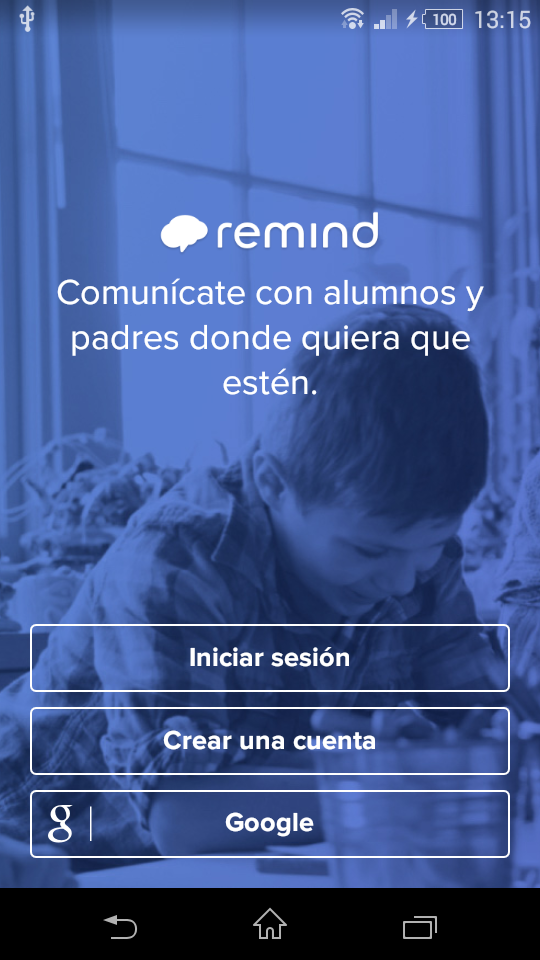
\includegraphics[scale=0.2]{Remind}
			\caption{Pantalla de bienvenida de la aplicación Remind}
			\label{fig:Remind}
		\end{figure}
		
		\subsubsection{miColegioApp}
		En {\it miColegioApp} \cite{4:micolegioapp:online} el usuario se registra como alumno, profesor, padre, madre, tutor legal o persona autorizada. Una vez registrado, se solicita el código al centro, que debe haber contratado los servicios de la empresa previamente, y se introduce en la aplicación. Cuando se ha asociado al usuario con un centro, el dueño del dispositivo recibirá notificaciones y circulares del colegio.
		En la figura \ref{fig:miColegioApp} se observa la pantalla de inicio.
		
		{\it CreaTáctil} \cite{24:creatactil:online} es una empresa de base tecnológica que ofrece soluciones personalizadas en el campo de la tecnología y la informática, con especialización en el desarrollo de aplicaciones multiplataforma.
		Persiguen convertirse en una referencia en el desarrollo de aplicaciones móviles.
		
		\begin{figure}[h !]
			\centering
			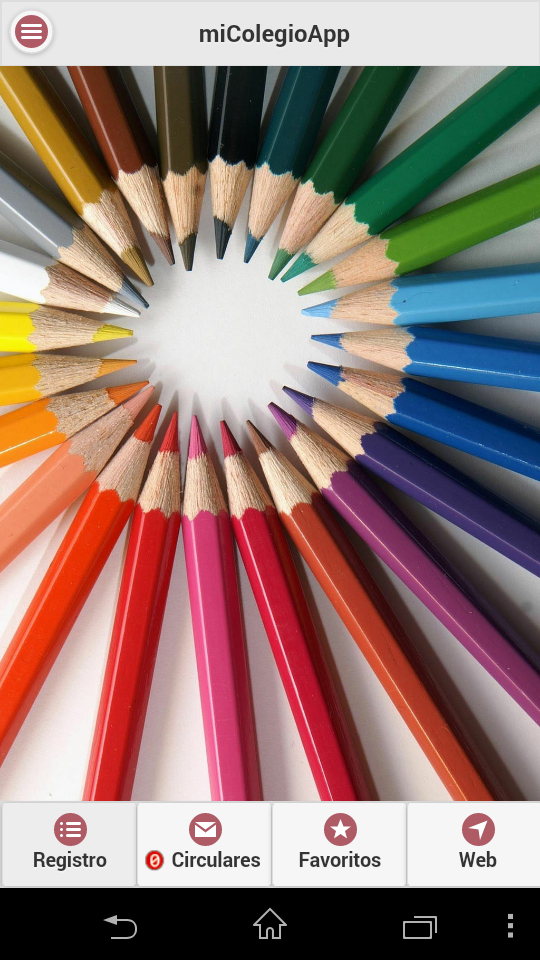
\includegraphics[scale=0.2]{miColegioApp}
			\caption{Pantalla de bienvenida de la Aplicación miColegioApp}
			\label{fig:miColegioApp}
		\end{figure}